\documentclass[xcolor=dvipsnames]{beamer}
\usepackage[utf8]{inputenc}
\usepackage{xcolor}
\usepackage{amsmath}
\usepackage{booktabs}
\definecolor{UBCblue}{rgb}{0.01, 0.55, 0.01}
\usetheme{Madrid}
\setbeamertemplate{caption}[numbered]
\usecolortheme[named=UBCblue]{structure}

\title[Pitch Efficiency]{Bayesian Hierarchical Model for Pitch Efficiency in Major League Baseball}
\author{Jacob Andros}
\date{December 7, 2021}

\begin{document}

\maketitle

%%%%%%%%%%%%%%%%%%%%%%%%%%%%%%%%%%%%%%%%%%%%%%%%%%%%%%%%%%%

\begin{frame}{Background}


\includegraphics[scale=0.63]{figs/pitchers.PNG}

\end{frame}

%%%%%%%%%%%%%%%%%%%%%%%%%%%%%%%%%%%%%%%%%%%%%%%%%%%%%%%%%%%

\begin{frame}{Model}

\noindent Level 1:
\begin{equation}
    y_{ij} | \theta_i \sim \text{Poisson}(\theta_i) \hspace{8pt}
    \label{eq:lv1}
\end{equation}
%\vspace{.1cm}

\noindent Level 2:
\begin{equation}
    \theta_i | a_i, \hspace{1pt} b_i \sim \text{Gamma}(a_i, \hspace{1pt} b_i)
    \label{eq:lv2}
\end{equation}
%\vspace{.1cm}

\noindent Level 3:
\begin{equation}
    a_i \sim \text{N}(16, 3) \hspace{.4cm} b_i \sim \text{N}(1, \frac{1}{16})
    \label{eq:lv3}
\end{equation}

\vspace{0.6cm}
$$
i \in \{1,2,3,4,5,6\}, \hspace{5pt} j \in \{1,\hdots,n_i\}
$$


\end{frame}

%%%%%%%%%%%%%%%%%%%%%%%%%%%%%%%%%%%%%%%%%%%%%%%%%%%%%%%%%%%

\begin{frame}{Computation}

{\footnotesize
\begin{align*}
    \begin{split}
        \text{P}(\boldsymbol{\theta}, \boldsymbol{a}, \boldsymbol{b} | \boldsymbol{y}) &\propto \text{P}(\boldsymbol{y} | \boldsymbol{\theta}) \text{P}(\boldsymbol{\theta}|\boldsymbol{a},\boldsymbol{b})\text{P}(\boldsymbol{a},\boldsymbol{b}) 
        \\
        &\propto \prod_{i=1}^6 \Big[\prod_{j=1}^{n_i} \big( \frac{\theta_i^{y_{ij}}e^{-\theta_i}}{y_{ij}!} \big) \big( \frac{b_i^{a_i}}{\Gamma(a_i)} \theta_i^{a_i-1}e^{-\theta_ib_i} \big) \exp\{-\frac{1}{2}(a_i-16)^2-\frac{1}{2}(b_i-1)^2 \} \Big] 
        \\
        &\propto \prod_{i=1}^6 \Big[ \frac{1}{\Gamma(a_i)} \theta_i^{a_i-1+\sum y_{ij}} e^{-n_i \theta_i} b_i^{a_i} \exp \{ -\theta_i b_i - \frac{1}{2}(a_i-16)^2 - \frac{1}{2}(b_i-1)^2 \} \Big]
        \\
        \text{P}(\boldsymbol{\theta} | \boldsymbol{a}, \boldsymbol{b}, \boldsymbol{y}) &\propto \prod_{i=1}^6 \Big[ \theta_i^{a_i-1+\sum y_{ij}} e^{-n_i \theta_i - b_i \theta_i} \Big] \propto \prod_{i=1}^6 \Big[ \theta_i^{a_i-1+\sum y_{ij}} e^{-n_i \theta_i - b_i \theta_i} \Big]
        \\
        &\Longrightarrow \theta_i | \; \cdot \sim \text{Gamma}(a_i + \sum_{j=1}^{n_i} y_{ij}, n_i+b_i)
        \label{eq:cond-theta}
    \end{split}
\end{align*}
}%

\end{frame}

%%%%%%%%%%%%%%%%%%%%%%%%%%%%%%%%%%%%%%%%%%%%%%%%%%%%%%%%%%%

\begin{frame}{Convergence}

\begin{figure}[h]
    \centering
    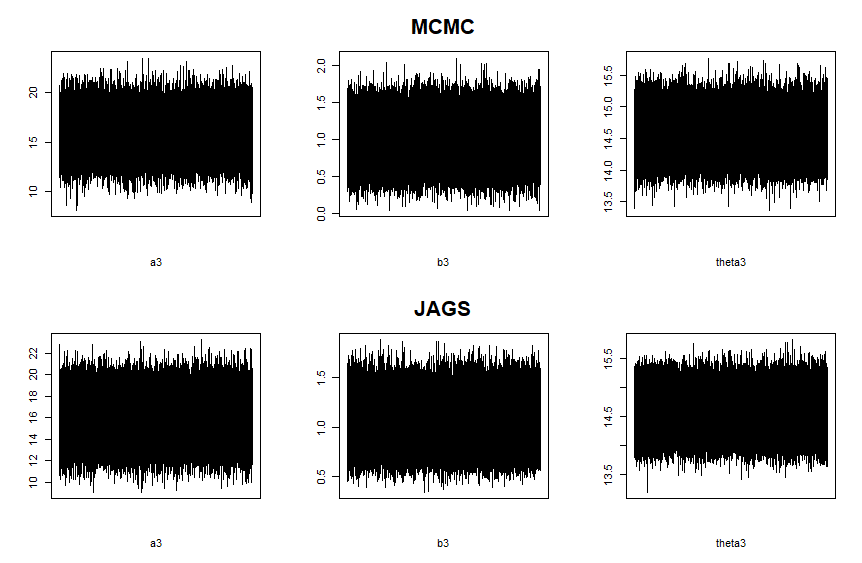
\includegraphics[scale=0.4]{figs/trace.png}
    \caption{Trace plots for Zack Wheeler ($a_3, b_3, \theta_3$) under each sampling method. The trace plots for the other 5 pitchers are comparable.}
    \label{fig:trace}
\end{figure}


\end{frame}

%%%%%%%%%%%%%%%%%%%%%%%%%%%%%%%%%%%%%%%%%%%%%%%%%%%%%%%%%%%

\begin{frame}{Convergence}

Better overall convergence and computational efficiency with JAGS, but both methods work.

\begin{table}[]
    \centering
    \begin{tabular}{lllllll}
    \toprule[1.5pt]
         & Parameters & Chains & Acceptance & ESS & Geweke & $\hat{R}$ \\
         \midrule
        MCMC & $\boldsymbol{a}$ & 1 & 0.55 & 32070 & .26 & NA \\
        & $\boldsymbol{b}$ & 1 & 0.28 & 50022 & .09 & NA \\
        & $\boldsymbol{\theta}$ & 1 & NA & 99673 & .09 & NA \\
        JAGS & $\boldsymbol{a}$ & 8 & NA & 158585 & .10 & 1 \\
        & $\boldsymbol{b}$ & 8 & NA & 158989 & 0.37 & 1 \\
        & $\boldsymbol{\theta}$ & 8 & NA & 159534 & .09 & 1 \\
        \bottomrule[1.5pt]
    \end{tabular}
    \caption{Convergence comparison between MCMC and JAGS}
\end{table}

\end{frame}

%%%%%%%%%%%%%%%%%%%%%%%%%%%%%%%%%%%%%%%%%%%%%%%%%%%%%%%%%%%

\begin{frame}{Comparison of JAGS with my MCMC}

\begin{table}[h]
    \centering
    {\tiny %
    \begin{tabular}{llccc}
         \hline
         \textbf{MCMC} & Pitcher & Posterior Median & 95\% Credible Interval & 95\% MC Interval \\
         \hline
         $\theta_1$ & Walker Buehler & 14.718 & (14.16, 15.29) & (14.71977, 14.71978) \\
         $\theta_2$ & Nathan Eovaldi & 15.543 & (14.94, 16.17) & (15.54786, 15.54787) \\
         $\theta_3$ & Zack Wheeler & 14.585 & (14.05, 15.13) & (14.58555, 14.58556) \\
         $\theta_4$ & Taijuan Walker & 14.682 & (14.05, 15.33) & (14.68592, 14.68593) \\
         $\theta_5$ & Shane McClanahan & 15.663 & (14.90, 16.44) & (15.66531, 15.66532) \\
         $\theta_6$ & Max Fried & 15.130 & (14.49, 15.78) & (15.13280, 15.13281) \\
         \hline
         \textbf{JAGS} & Pitcher & Posterior Median & 95\% Credible Interval & 95\% MC Interval \\
         \hline
         $\theta_1$ & Walker Buehler & 14.713 & (14.16, 15.29) & (14.71576, 14.71576) \\
         $\theta_2$ & Nathan Eovaldi &  15.543 & (14.94, 16.16) & (15.54521, 15.54522) \\
         $\theta_3$ & Zack Wheeler & 14.580 & (14.05, 15.13) & (14.58233, 14.58234) \\
         $\theta_4$ & Taijuan Walker & 14.677 & (14.04, 15.33) & (14.68056, 14.68057) \\
         $\theta_5$ & Shane McClanahan & 15.660 & (14.91, 16.44) & (15.66372, 15.66373) \\
         $\theta_6$ & Max Fried & 15.128 & (14.50, 15.78) & (15.13112, 15.13112) \\
         \hline
    \end{tabular}
    }%   
    \caption{Posterior summarization under each method. The medians and credible intervals are virtually identical.}
    \label{tab:bayes-ests}
\end{table}

\end{frame}

%%%%%%%%%%%%%%%%%%%%%%%%%%%%%%%%%%%%%%%%%%%%%%%%%%%%%%%%%%%

\begin{frame}{Comparison of JAGS with my MCMC}

\begin{figure}[h]
    \centering
    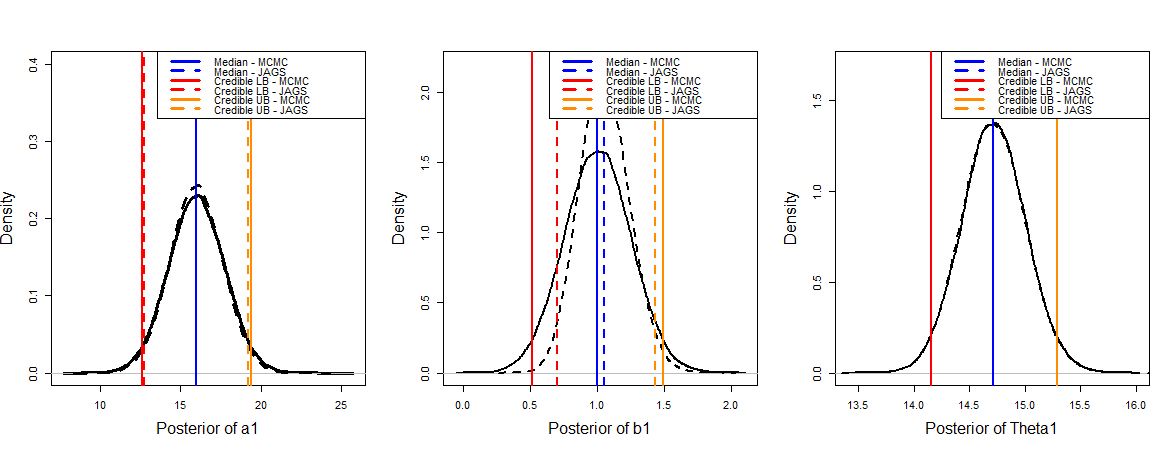
\includegraphics[scale=0.38]{figs/comp.png}
    \caption{Posterior densities of $a_1$, $b_1$, and $\theta_1$ which corresponds to Walker Buehler. Monte Carlo error bounds are not plotted because they are visually no different from the point estimates.}
    \label{fig:buehler}
\end{figure}

\end{frame}

%%%%%%%%%%%%%%%%%%%%%%%%%%%%%%%%%%%%%%%%%%%%%%%%%%%%%%%%%%%

\begin{frame}{Posterior Densities}

\begin{figure}
    \centering
    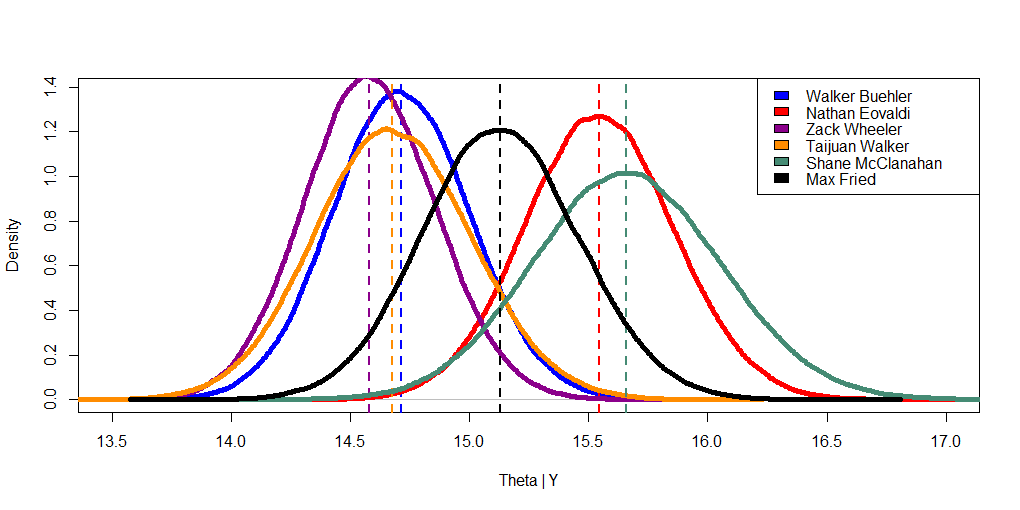
\includegraphics[scale=0.45]{figs/posterior.png}
    \caption{Posterior densities and medians of ($\theta_1, \hdots, \theta_6 | \boldsymbol{a}, \boldsymbol{b}, \boldsymbol{y}$) }
    \label{fig:post}
\end{figure}


\end{frame}

%%%%%%%%%%%%%%%%%%%%%%%%%%%%%%%%%%%%%%%%%%%%%%%%%%%%%%%%%%%

\begin{frame}{Sensitivity Analysis}

Alternative Priors:
\begin{align*}
    \begin{split}
        \textbf{1) } \theta_i &\sim \text{Gamma}(a_i, b_i); \hspace{4pt} a_i \sim \text{N}(16, 1); \hspace{4pt} b_i \sim \text{N}(1,0.01) \\
        \textbf{2) } \theta_i &\sim \text{Gamma}(a_i, b_i); \hspace{4pt} a_i \sim \text{N}(32, 3); \hspace{4pt} b_i \sim \text{N}(2,\frac{1}{16}) \\
        \textbf{3) } \theta_i &\sim \text{N}(a_i, b_i); \hspace{4pt} a_i \sim \text{Unif}(14,17); \hspace{4pt} b_i \sim \text{Unif}(0.1, 1) 
    \end{split}
\end{align*}

\end{frame}

%%%%%%%%%%%%%%%%%%%%%%%%%%%%%%%%%%%%%%%%%%%%%%%%%%%%%%%%%%%

\begin{frame}{Sensitivity Analysis}

\begin{figure}[h]
    \centering
    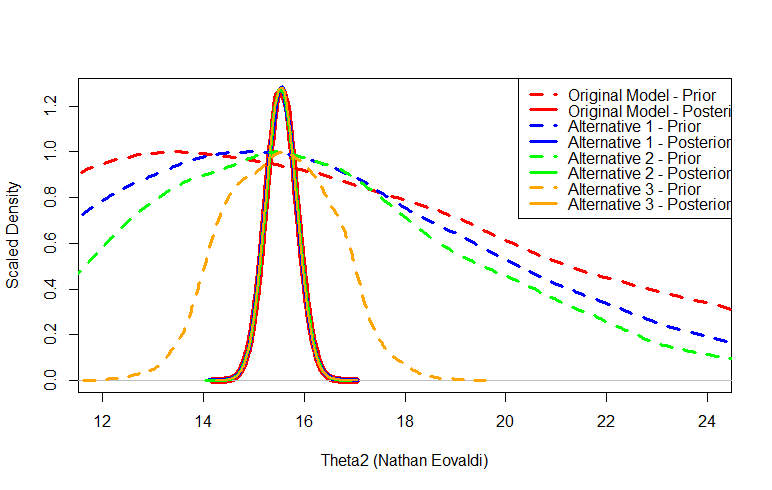
\includegraphics[scale=0.45]{figs/sensitivity.png}
    \caption{Four different prior distributions on $\theta_2$ and their resulting posteriors. $\theta_2$ corresponds to Nathan Eovaldi. }
    \label{fig:sens}
\end{figure}

\end{frame}

%%%%%%%%%%%%%%%%%%%%%%%%%%%%%%%%%%%%%%%%%%%%%%%%%%%%%%%%%%%

\begin{frame}{Comparison to Frequentist Methods}

Casella and Berger (2001) used the sufficient statistic $W=\sum y_i$ to obtain the formula for a $(1-\alpha)$\% confidence interval on $\theta$ in the Poisson distribution.

\begin{equation*}
    \Big\{ \theta: \; \frac{1}{2n}\chi^2_{W,1-\alpha/2} \leq \theta \leq 
    \frac{1}{2n} \chi^2_{2(W+1),\alpha/2} \Big\}
\end{equation*}

\end{frame}

%%%%%%%%%%%%%%%%%%%%%%%%%%%%%%%%%%%%%%%%%%%%%%%%%%%%%%%%%%%

\begin{frame}{Comparison to Frequentist Methods}

\begin{table}[h]
    \centering
    \begin{tabular}{lccc}
         \hline
         Pitcher & Parameter & Sample Mean & 95\% Confidence Interval \\
         \hline
         Walker Buehler & $\theta_1$ & 14.713 & (14.16, 15.29) \\
         Nathan Eovaldi & $\theta_2$ &  15.544 & (14.94, 16.17) \\
         Zack Wheeler & $\theta_3$ & 14.579 & (14.04, 15.13) \\
         Taijuan Walker & $\theta_4$ & 14.676 & (14.04, 15.33) \\
         Shane McClanahan & $\theta_5$ & 15.663 & (14.90, 16.45) \\
         Max Fried & $\theta_6$ & 15.128 & (14.49, 15.78) \\
         \hline
    \end{tabular}
    \caption{Point and interval estimates for $\theta_1, \hdots, \theta_6$ using maximum likelihood and the Poisson 95\% confidence interval.}
\end{table}

\end{frame}

%%%%%%%%%%%%%%%%%%%%%%%%%%%%%%%%%%%%%%%%%%%%%%%%%%%%%%%%%%%

\begin{frame}{Applications in Prediction}

1) Predict the number of pitches thrown in a new inning for one of the pitchers from the study.

\begin{figure}[h]
    \centering
    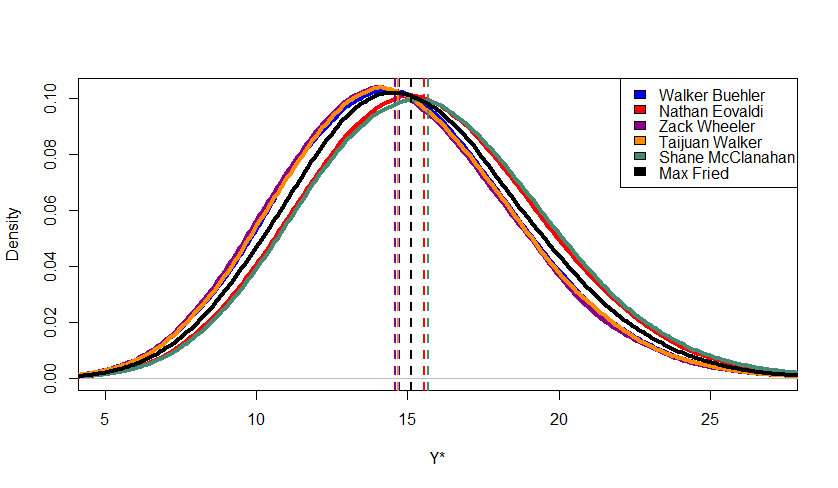
\includegraphics[scale=0.35]{figs/preds.png}
    \caption{Posterior predictive density for each pitcher. This predictive density is perhaps the most useful application of the analysis to baseball teams and managers. The dotted lines now represent the means rather than the medians, since the median would be exactly 15 for most of the pitchers and would not convey much information visually.}
    \label{fig:preds}
\end{figure}

\end{frame}

%%%%%%%%%%%%%%%%%%%%%%%%%%%%%%%%%%%%%%%%%%%%%%%%%%%%%%%%%%%

\begin{frame}{Applications in Prediction: Example}

The manager of the Tampa Bay Rays has Shane McClanahan at 90 pitches after 5 innings, and is trying to decide whether to send him out for the sixth. His predictive distribution could be used to estimate the probability of completing the next inning in 10 pitches or less (so as to keep him at the 100 pitch limit). In his case, this probability is estimated at 9.05\%. On the other hand, the Phillies could be a little more optimistic about Zack Wheeler, for whom this probability is 14.18\%.
    
\end{frame}

%%%%%%%%%%%%%%%%%%%%%%%%%%%%%%%%%%%%%%%%%%%%%%%%%%%%%%%%%%%

\begin{frame}{Applications in Prediction}

2) Predict the rate parameter $\theta_j$ for a new pitcher or the number of pitches they throw in a new inning.

\begin{figure}[h]
    \centering
    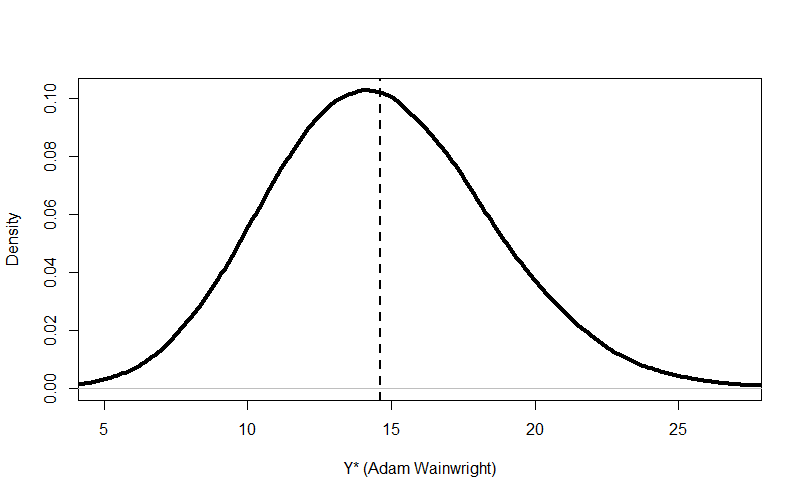
\includegraphics[scale=0.37]{figs/ww.png}
    \caption{The posterior predictive density for Adam Wainwright of the St. Louis Cardinals, another Tommy John comeback pitcher. His average projected P/IP falls in between that of Zack Wheeler and Taijuan Walker, so he appears to be quite efficient with his pitches.}
    \label{fig:ww}
\end{figure}


\end{frame}

%%%%%%%%%%%%%%%%%%%%%%%%%%%%%%%%%%%%%%%%%%%%%%%%%%%%%%%%%%%

\begin{frame}{Applications of the Hyperparameters}

Can be used to understand the nature of the distribution of P/IP for any pitcher.\\
\vspace{0.5cm}
\textbf{Example:} \\
$\hat{a}_5 = 16.06, \hat{b}_5 = 1.02$ (Shane McClanahan) \\
$\hat{a}_3 = 15.96, \hat{b}_3 = 1.05$ (Zack Wheeler) \\
\vspace{0.5cm}
$\Longrightarrow$ More uncertainty in prediction/inference on the pitch count for McClanahan than for Wheeler.


\end{frame}

%%%%%%%%%%%%%%%%%%%%%%%%%%%%%%%%%%%%%%%%%%%%%%%%%%%%%%%%%%%

\begin{frame}{Conclusion}

\begin{itemize}
    \item Samples can be drawn from a posterior predictive distribution for any given pitcher in Major League Baseball.
        \begin{itemize}
            \item Establishes a direct application to baseball teams trying to determine the longevity and efficiency of their starters.
        \end{itemize}
    \item Every pitcher is different due to a variety of factors (as is every pitcher's individual start).
    \begin{itemize}
        \item Age, climate, team, opposing team, health history, etc.
        \item Future models could incorporate data on some of these covariates to assess mathematical relationships (instead of being predictive only).
    \end{itemize}
    
\end{itemize}



\end{frame}


\end{document}
